\documentclass[11pt]{article}

% ---------- Packages ----------
\usepackage[margin=1in]{geometry}
\usepackage{graphicx}
\usepackage{booktabs}
\usepackage{tabularx}
\usepackage{natbib}
\usepackage{hyperref}
\usepackage{tikz}
\usetikzlibrary{arrows.meta, positioning, shapes.geometric, fit, calc}
\usepackage{enumitem}
\usepackage{float}
\usepackage{verbatim}
\hypersetup{colorlinks=true, linkcolor=blue, citecolor=blue, urlcolor=blue}

% ---------- Metadata ----------
\title{Transparent Control: A Practical Guide to Agentic AI for Social Science Research}
\author{Simone Paci\thanks{Stanford University. \texttt{spaci@stanford.edu}}}
\date{April 2026}

\begin{document}

\maketitle

\begin{abstract}
Research practice in social science has shifted sharply around agentic AI over the past year, yet adoption has outrun a shared understanding of what effective and responsible use looks like. This paper offers a working manual rather than a forecast. It develops a minimum vocabulary for the agentic-AI landscape, builds a layered workflow that moves from tool choice through harness, context, and prompt engineering into agent management across the research process, and proposes governance principles for reporting. Two principles run throughout: \emph{researcher control}, which keeps every substantive decision with the human, and \emph{radical transparency}, which expands the replication package to include the inputs, throughputs, and outputs of the AI-assisted process itself. These principles are implementable today using the same infrastructure the paper recommends, and implementing them is the precondition for trust in agentic research workflows.
\end{abstract}

% =====================================================================
\section{Introduction}
\label{sec:intro}
% Target: 3 paragraphs. Short, argumentative, narrowing from stakes to
% claim. No throat-clearing. No generic relevance talk.

\paragraph{Motivation.}
In the space of a few months, a growing share of social scientists have restructured the day-to-day of their work around agentic AI. Recent surveys put researcher adoption of AI tools at 84 percent, but only about a quarter of that use runs through purpose-built research tooling rather than consumer chat interfaces \citep{wiley2025adoption}; in parallel, AI-tagged publications in the natural, physical, and life sciences are growing at 26 to 28 percent year over year \citep{hai2026aiindex}. The frontier is wider still. Agentic pipelines now run routine empirical work end to end, from data cleaning through heterogeneous-treatment sweeps to publication-ready tables \citep{pepinsky2026agentic}, and platforms built around agent orchestration are beginning to automate portions of the research process itself, from question formulation through analysis \citep{sresearcher2026}. Uptake has outrun understanding. The deeper problem is epistemic: when an agent drafts, runs, or interprets, the ordinary anchors of authorship and replicability no longer sit where researchers assume they do.

\paragraph{Positioning.}
Against a growing body of work that frames AI's implications for social science in programmatic or speculative terms, this paper takes the most concrete approach available: a working manual rather than a forecast. It installs the vocabulary a researcher needs to reason about the agentic landscape precisely, rather than gesturally. It then builds a layered workflow that runs from tool choice through prompt-level practice and into agent-level management, so the reader can construct a research routine instead of improvising one. It closes with governance principles for reporting that any individual researcher can implement without waiting for disciplinary consensus.

\paragraph{Core principles.}
Running through both the workflow and the governance claims are two principles the paper argues should govern AI adoption in research: researcher control and radical transparency. The first holds that every substantive decision in a project, from framing and citation through phrasing and final sign-off, must remain with the researcher; automation belongs at the level of execution, not at the level of judgment. The second holds that the burden of credibility has shifted: releasing data and code is no longer sufficient, and a credible replication package must extend to the inputs, throughputs, and outputs of the AI-assisted process itself. Section~\ref{sec:conclusions} returns to these principles when it takes up the risks the paper leaves on the table.

% =====================================================================
\section{The AI Vocabulary}
\label{sec:vocabulary}

Using AI effectively starts with being able to name what is being used. The rest of this section installs the minimum vocabulary the workflow in Section~\ref{sec:deploy} will assume, organized into two layers: the objects themselves, and the engineering layers at which a researcher designs how those objects are deployed.

\subsection{Fundamentals}
\label{sec:vocab-fundamentals}

The relevant object is generative AI rather than AI broadly construed. Generative models produce text, code, and images from a prompt, and occupy a narrow slice of the wider field that also houses predictive modeling and classical machine learning. The practical shift in 2026, however, is not to generative models as such but to \emph{agentic} generative AI: models wired into a runtime that lets them call tools, read and write files, execute code, and loop until a task is done. Non-agentic chat was useful but bounded; agentic systems shift the model from answer-machine to actor, and that shift is what opened the research-workflow inflection described in Section~\ref{sec:intro}.

A session with any such system is a \emph{model-instance} with a bounded \emph{context window}. Performance is not uniform across that window: as context fills, the model becomes less reliable, and long-running tasks therefore require either compaction (summarizing earlier turns into a condensed record) or a planned restart. Researchers who ignore this constraint discover it through drifted outputs and silent errors deep in a session. The corollary is that complex work is best split across multiple instances rather than crammed into one, and the practice increasingly organizes itself around \emph{swarms}: a parent agent dispatches scoped tasks to child instances with fresh context and then integrates the results.

Two reliability failure modes deserve separate names. False-positive errors are confidently fabricated outputs: a citation that does not exist, a variable that was not in the dataset, a fact that was never in the source. These are conspicuous, and researchers tend to brace for them. False-negative errors are quieter: information that was present in a document the agent had access to, but was missed or never surfaced. The second mode is harder to catch and arguably the more dangerous in research contexts, because what is wrong is what is absent.

A useful way to hold all of this together is the metaphor of an extremely capable research assistant. Blindfolded, with pen and paper, that RA accomplishes little; equipped with clear instructions, a working laptop, and a curated library of methods texts and prior work, the same person becomes a serious collaborator. Agents are no different. They need the scaffolding a researcher can provide, and the rest of this paper is about how to provide it.

\subsection{Key Components}
\label{sec:vocab-components}

The best-practice frontier has moved in three stages, each adding a layer rather than replacing the previous one. The first stage, which coincided with the public arrival of ChatGPT, was \emph{prompt engineering}: craft the instruction well enough and the model will do the task. That skill remains necessary, but as context windows have grown the binding constraint has shifted outward. What now separates a useful session from a failed one is \emph{context engineering}, the curation of which files, prior turns, reference documents, and scratch space the model can see at any given moment. A third frontier has opened more recently around the runtime itself. \emph{Harness engineering} is the design of the tools, skills, permissions, and control loops available before any single prompt is written. Each layer conditions the ones below it, which is why Section~\ref{sec:deploy} takes them in that order.

Two objects do most of the customization work inside the harness. A \emph{skill} is a reusable, named procedure that an agent can invoke on demand: a short playbook encoding the researcher's preferred method for a recurring task. \emph{Orchestration} is the researcher's overall design for how tasks are broken across instances, subagents, and skills over the course of a project. Together, they are the layer at which a generic model becomes a particular researcher's collaborator, and where most of the practical leverage now sits.

Table~\ref{tab:vocabulary} summarizes the ten concepts above.
% Table 1 — Key vocabulary for agentic AI in social-science research
% Requires: \usepackage{booktabs}, \usepackage{tabularx}, \usepackage{float}
% Draft v2 (2026-04-21): tightened text ~30%, anchored with [H].

\begin{table}[H]
\centering
\small
\begin{tabularx}{\textwidth}{@{}lXX@{}}
\toprule
\textbf{Concept} & \textbf{Definition} & \textbf{Example} \\
\midrule
\multicolumn{3}{@{}l}{\emph{Fundamentals}} \\
\addlinespace
Generative AI (GenAI) & Models that produce text, code, or images from a prompt. A narrow slice of the wider AI umbrella, which also houses predictive and classical ML. & ChatGPT drafting a literature summary. \\
\addlinespace
Agentic AI & A GenAI model wired into a runtime that lets it call tools, read and write files, execute code, and loop until a task is done. & Claude Code opening a repo, editing files, running tests, and iterating without re-prompting. \\
\addlinespace
Model-instance & One stateful session of a model with a bounded \emph{context window}. Performance degrades as the window fills; long tasks need \emph{compaction} or a restart. & A session nearing its context limit compacts earlier turns and continues. \\
\addlinespace
Subagent / agent swarm & A parent agent spawns child instances with scoped tasks and fresh context, then integrates their outputs. & A research-lead agent dispatching parallel search subagents, one per literature strand. \\
\addlinespace
Hallucination & Confident but fabricated or misremembered output. Two modes: \emph{false positives} (invented citation, variable, or fact) and \emph{false negatives} (information present but missed). & Citing a paper that does not exist; missing a footnote in a document the agent has seen. \\
\addlinespace
\midrule
\multicolumn{3}{@{}l}{\emph{Engineering layers}} \\
\addlinespace
Prompt engineering & Crafting the instruction given to a model for a single task. Still necessary, no longer sufficient. & Specifying role, task, format, and worked examples for a classification job. \\
\addlinespace
Context engineering & Curating what the model can see: which files, prior turns, reference documents, and scratch space are visible at any moment. & A project folder with README, roadmap, background notes, and archive pattern, so any session starts with the right material at hand. \\
\addlinespace
Harness engineering & Designing the runtime around the model: which tools, skills, permissions, and control loops exist before any prompt is written. & Choosing Claude Code over a bare chat; configuring allowed shell commands and available skills. \\
\addlinespace
Skill & A reusable, named procedure an agent can invoke on demand, encoding the researcher's preferred method for a recurring task. & A \texttt{lit-review-protocol} skill standardizing how every literature search is run, logged, and classified. \\
\addlinespace
Orchestration & The researcher's design for how tasks are split and routed across instances, subagents, and skills over a project. & One instance per section, subagents per literature strand, a shared skills library, a running interaction log. \\
\bottomrule
\end{tabularx}
\caption{Key concepts of agentic AI for social-science research. The upper block introduces what the objects \emph{are}; the lower block introduces the layers at which a researcher designs \emph{how they are used}.}
\label{tab:vocabulary}
\end{table}


% =====================================================================
\section{How to Deploy AI Effectively}
\label{sec:deploy}

The setup stack is five layers deep, and each layer conditions the ones below it. Tool choice determines which harnesses can exist on top; the harness determines which skills, permissions, and tools the agent can reach; context engineering determines what that agent can see inside a given project; the prompt determines what the agent does with what it sees; and agent management determines how all of this gets reviewed and integrated across the research process. Figure~\ref{fig:setup-flow} shows the stack. The remainder of this section takes the layers in order.

\begin{figure}[t]
  \centering
  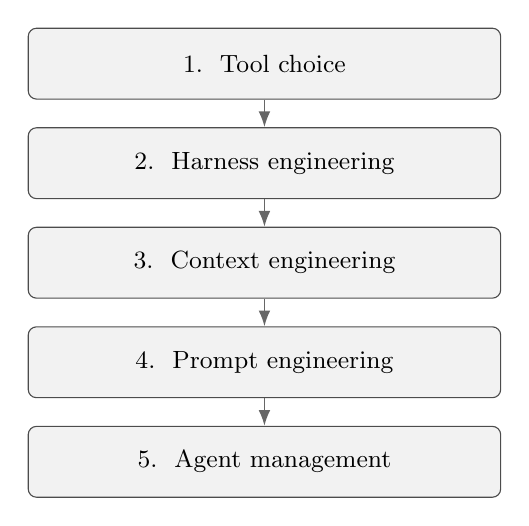
\begin{tikzpicture}[
    node distance=0.35cm,
    layer/.style={rectangle, rounded corners=3pt, draw=black!70, fill=black!5, minimum width=6cm, minimum height=0.9cm, align=center, font=\small},
    arr/.style={-Latex, draw=black!60, line width=0.6pt}
  ]
    \node[layer] (tool) {1.~~Tool choice};
    \node[layer, below=of tool] (harness) {2.~~Harness engineering};
    \node[layer, below=of harness] (context) {3.~~Context engineering};
    \node[layer, below=of context] (prompt) {4.~~Prompt engineering};
    \node[layer, below=of prompt] (agent) {5.~~Agent management};
    \draw[arr] (tool) -- (harness);
    \draw[arr] (harness) -- (context);
    \draw[arr] (context) -- (prompt);
    \draw[arr] (prompt) -- (agent);
  \end{tikzpicture}
  \caption{The setup stack. Each layer conditions the ones below: tool choice shapes the harness, the harness shapes the context, the context shapes what can be prompted, and the prompt shapes how agents are managed across a research project.}
  \label{fig:setup-flow}
\end{figure}

\subsection{Choice of Toolset}
\label{sec:deploy-toolset}

The first choice is where the agent lives. The current landscape offers several viable research harnesses, including Claude Code, Codex, Antigravity, and various IDE plug-ins for VS~Code and terminal-based environments. Behind those harnesses sit at least three frontier providers in active competition, and the capability frontier has shifted several times in the last year alone. Committing a research workflow to a single provider is therefore fragile, and the more durable choice is to build practices that survive a model swap.

A second, less visible choice sits alongside the first. Closed-weights models remain at or near the frontier on most benchmarks, with open-weights models trailing by a modest margin \citep{hai2026aiindex}. The gap narrows once replicability enters the picture. As Spirling and others have argued, research that leans on a commercial closed-weights model is effectively unreplicable once the vendor updates or retires that model; no amount of careful prompt logging recovers what the vendor has removed \citep{spirling2023opensource, spirling2026talks}. Open-weights models can be versioned, archived, and rerun. For any result meant to travel beyond proof-of-concept, that property is not a luxury.

\subsection{Harness Engineering}
\label{sec:deploy-harness}

A harness is the runtime scaffolding inside which an agent operates: the tools it can call, the skills it can invoke, the permissions it has, and the control loops that bound its behavior. Setting up a harness well is the highest-leverage investment a researcher can make, because every prompt thereafter inherits from it.

The central artifact inside a harness is the skill library. A \emph{skill} captures a researcher's preferred approach to a recurring task in a named, reusable form, so that invoking the skill is equivalent to reactivating a prior conversation about method. Skills should be built from two inputs together rather than from either alone: trusted sources (textbooks, methods papers, the researcher's prior work) and a self-interview that elicits the researcher's actual preferences and constraints. Figure~\ref{fig:skill-build} illustrates the pattern. The self-interview is what prevents the skill from defaulting to a textbook-average approach when the researcher has idiosyncratic judgments worth preserving. Once built, skills are loaded on demand rather than stuffed into context up front, because unfolding a skill only when it is needed preserves context for the work itself.

\begin{figure}[t]
  \centering
  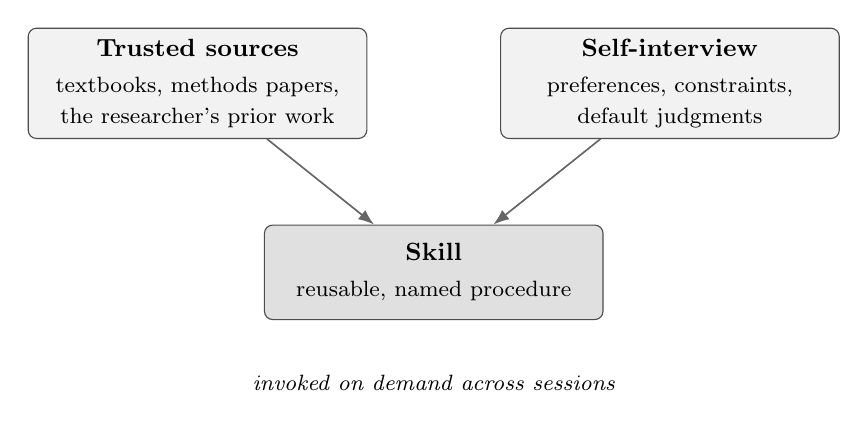
\begin{tikzpicture}[
    box/.style={rectangle, rounded corners=3pt, draw=black!70, fill=black!5, minimum width=4.3cm, minimum height=1.4cm, align=center, font=\small},
    skillbox/.style={rectangle, rounded corners=3pt, draw=black!70, fill=black!12, minimum width=4.3cm, minimum height=1.2cm, align=center, font=\small},
    arr/.style={-Latex, draw=black!60, line width=0.6pt}
  ]
    \node[box] (sources) at (-3, 0) {\textbf{Trusted sources}\\[2pt] \footnotesize textbooks, methods papers,\\ \footnotesize the researcher's prior work};
    \node[box] (interview) at (3, 0) {\textbf{Self-interview}\\[2pt] \footnotesize preferences, constraints,\\ \footnotesize default judgments};
    \node[skillbox] (skill) at (0, -2.4) {\textbf{Skill}\\[2pt] \footnotesize reusable, named procedure};
    \node[font=\footnotesize\itshape] at (0, -3.8) {invoked on demand across sessions};
    \draw[arr] (sources) -- (skill);
    \draw[arr] (interview) -- (skill);
  \end{tikzpicture}
  \caption{Building a skill. Trusted sources and a self-interview converge into a named, reusable procedure that the agent invokes on demand. A diff-in-differences skill, for example, combines a methods-text specification of the estimator with the researcher's own answers about how to handle clustering, event-time windows, and the reporting format for parallel-trends diagnostics.}
  \label{fig:skill-build}
\end{figure}

Alongside skills, a harness should carry tools and workflows: library stubs that standardize which packages the agent reaches for, orchestration patterns for decomposing complex tasks, and engagement rules that tell the agent when to pause and ask rather than improvise. A final discipline is the verbosity check: three passes on any non-trivial agent output, one that strips scaffolding, one that compresses what remains, and one that verifies the claims the compression made possible. The three roles can be filled by separate subagents or by the researcher directly, but skipping the last is how fabrications survive into a draft.

\subsection{Context Engineering}
\label{sec:deploy-context}

Once the harness is in place, the remaining question is what the agent should see. Context engineering treats the project as a sandbox repository: a single folder that carries all the relevant knowledge for the project, including background concepts, literature, data, scripts, and feedback. A session that begins inside such a folder inherits the project's full state; a session that begins with ad hoc paste-ins inherits whatever the researcher happened to attach.

Two kinds of artifact make this work. The first are orchestration artifacts: a README that states the rules of engagement, an implementation roadmap that functions as a living to-do list, and archive subfolders that absorb obsolete material rather than letting it accumulate. These keep the repository legible to any agent instance that enters it, including across long projects in which the researcher's own memory has faded. The second are transparency artifacts. Every major asset in the folder should be recorded in an asset registry that flags it as human-produced, agent-produced, or mixed, along with a verification status ranging from not-verified through partially-verified to human-verified. Every non-trivial agent session should be summarized in an interaction log that records date, researcher input, agent output, and model metadata. An emerging line of work on cryptographic authentication of research artifacts suggests these logs could eventually carry stronger guarantees \citep{gordon2025datanomad}, but even the simpler CSV-based version already delivers what a reviewer needs: a reconstructible record of the AI's role.

A \emph{project-setup skill} bundles the whole scaffold into a single invocation, so a new project can be instantiated in minutes rather than days. The folder housing this paper is the worked example. Figure~\ref{fig:project-setup} renders its directory tree alongside the workflows layered on top.

\begin{figure}[t]
  \centering
  \begin{minipage}[t]{0.46\textwidth}
    \vspace{0pt}
    \centering
{\footnotesize\ttfamily\raggedright
project/\\
\hspace*{1em}README.md\\
\hspace*{1em}implementation-roadmap.md\\
\hspace*{1em}asset-registry.csv\\
\hspace*{1em}interaction-log.csv\\
\hspace*{1em}background/\\
\hspace*{2em}literature/\\
\hspace*{2em}concepts/\\
\hspace*{2em}feedback/\\
\hspace*{2em}archive/\\
\hspace*{1em}drafts/\\
\hspace*{1em}figures/\\
\hspace*{1em}tables/\\
\hspace*{1em}scripts/\\
\hspace*{1em}appendix/\\
\par}
  \end{minipage}%
  \hfill
  \begin{minipage}[t]{0.50\textwidth}
    \vspace{0pt}
    \footnotesize
    \textbf{Supporting workflows}
    \begin{itemize}[leftmargin=*, itemsep=3pt, topsep=4pt]
      \item \emph{Verification flags} on every major asset: \texttt{not-verified}, \texttt{partially-verified}, \texttt{human-verified}.
      \item \emph{Provenance flags}: \texttt{human}, \texttt{agent}, or \texttt{mixed} for each asset entry.
      \item \emph{Interaction log} summarizing every non-trivial agent session (date, input, output, model metadata).
      \item \emph{Archive pattern}: obsolete files move to a local \texttt{archive/} rather than being deleted.
      \item \emph{Project-setup skill}: scaffolds the structure above in a single invocation.
    \end{itemize}
  \end{minipage}
  \caption{A sample project setup. Left: the directory layout that carries project knowledge into any new agent session. Right: the transparency and orchestration workflows layered on top of the directory.}
  \label{fig:project-setup}
\end{figure}

\subsection{Prompt Engineering}
\label{sec:deploy-prompt}

Once the harness, skills, and project scaffold are in place, the prompt itself becomes a smaller lever but still a necessary one. The first rule is one instance, one task. Long-running sessions that mix unrelated work accumulate context drift, cross-contaminate reasoning, and make review harder. A fresh instance for each discrete task is cheaper than the debugging that multi-purpose sessions invite.

The second rule is that the agent will invent a method unless one is provided, and the method it invents will be shaped by priors the researcher cannot easily audit. A prompt that does not specify how a task should be done is a prompt that delegates method to the model. The design of the plan is therefore the substantive work, not a preliminary. A good plan is goal-oriented, articulated before the agent begins executing, and refined through self-interview questions the researcher answers in advance rather than letting the agent fill in silently. Subplans for each major stage are usually worth the few minutes they take to write, because they replace a long and drifting session with a sequence of short accountable ones.

The third rule is that deterministic validation checks are worth more than any amount of model self-report. Where a type check, unit test, reference count, or schema validation exists, it should be wired in; the agent's claim to have verified its own output is not a substitute. This discipline matters most where the failure is quiet rather than loud, which is the common case in social-science empirics.

\subsection{Agent Management across the Research Process}
\label{sec:deploy-agents}

Agent integration is not a single decision made at the top of a project; it is a sequence of decisions made at every stage of the research process. Figure~\ref{fig:stages} maps the stages against candidate applications. At the question-formulation stage, agents help scope literatures, surface adjacent work, and stress-test framings. At the theory stage, they trace implications of assumptions, generate alternative derivations, and catch internal inconsistencies. At the empirical stage, they implement analysis pipelines, run specification sweeps, and produce publication-ready tables and figures. At the writing and presentation stage, they draft, edit, compress, and convert between formats.

\begin{figure}[t]
  \centering
  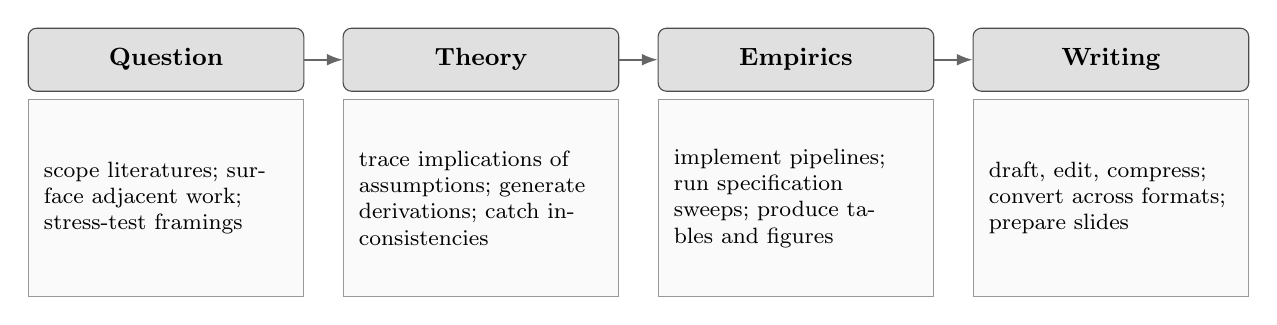
\begin{tikzpicture}[
    stage/.style={rectangle, rounded corners=3pt, draw=black!70, fill=black!12, minimum width=3.5cm, minimum height=0.8cm, align=center, font=\small\bfseries},
    app/.style={rectangle, draw=black!40, fill=black!2, minimum width=3.5cm, minimum height=2.5cm, align=left, text width=3.1cm, font=\footnotesize, inner sep=5pt, anchor=north},
    arr/.style={-Latex, draw=black!60, line width=0.6pt}
  ]
    \node[stage] (s1) at (0, 0) {Question};
    \node[stage] (s2) at (4, 0) {Theory};
    \node[stage] (s3) at (8, 0) {Empirics};
    \node[stage] (s4) at (12, 0) {Writing};
    \node[app] (a1) at (0, -0.5) {scope literatures; surface adjacent work; stress-test framings};
    \node[app] (a2) at (4, -0.5) {trace implications of assumptions; generate derivations; catch inconsistencies};
    \node[app] (a3) at (8, -0.5) {implement pipelines; run specification sweeps; produce tables and figures};
    \node[app] (a4) at (12, -0.5) {draft, edit, compress; convert across formats; prepare slides};
    \draw[arr] (s1) -- (s2);
    \draw[arr] (s2) -- (s3);
    \draw[arr] (s3) -- (s4);
  \end{tikzpicture}
  \caption{Research stages and candidate AI applications. Integration is a set of decisions at every stage, each subject to the review disciplines described below.}
  \label{fig:stages}
\end{figure}

Three review disciplines run across all of these stages. The first is chain-of-thought review: inspect the agent's reasoning, not only the final output. A correct answer reached through flawed reasoning fails differently than a wrong answer reached through plausible reasoning, and the difference matters for whether the result can be trusted downstream. The second is intermediate-step review: catch drift before it compounds, because an error introduced at step three of a ten-step pipeline is much cheaper to fix there than at step ten. The third is final review of finalized output: every claim the paper makes should be re-read and signed off by the researcher. These disciplines are the operational face of the control principle from Section~\ref{sec:intro}.

% =====================================================================
\section{Conclusions}
\label{sec:conclusions}

The workflow is only half the argument. The other half is what it implies about risk, about reporting, about institutional practice, and about the direction of the field.

\subsection{Risks and Ethics}
\label{sec:risks}

Every practical recommendation in this paper is also a claim about risk, and the two governing principles map onto the two risks the paper engages most directly. A third cluster is named but left open.

The first risk is to researchers themselves. Agents can do almost every operational task involved in producing a paper, and that possibility invites a slow erosion of the underlying skills. There is already suggestive evidence that heavy use of generative AI during learning can produce illusions of competence that mask real deficits \citep{prather2024widening}. The control principle is the answer: a researcher who retains substantive ownership of framing, measurement, interpretation, and phrasing continues to exercise the capacities that produced their ability to supervise in the first place. Automation belongs at the level of execution; intellectual control belongs with the researcher.

The second risk is to the reliability of results. Agentic tools lower the cost of specification search and multiverse-style exploration \citep{steegen2016multiverse, simmons2011falsepositive}, which means the ceiling on undisclosed p-hacking rises even if no individual researcher behaves worse than before. The transparency principle is the answer: if every step of the AI-assisted process is logged and reviewable, the space for undisclosed search collapses. Transparency is the condition under which agentic workflows can be trusted in the first place.

A third cluster of risks is flagged here but left open. Agentic workflows compress research timelines in ways that may erode the slow, deep thinking social-science training has long relied on, and this paper offers no principled way to calibrate the trade-off between speed and depth. Uneven adoption is likely to widen productivity gaps between researchers and institutions \citep{mohammadi2026reshaping, chugunova2026germany}, though the relatively low marginal cost of frontier subscriptions offers a partial democratizing countercurrent. Environmental externalities, privacy exposures, and the broader societal consequences of automating knowledge work are real, important, and beyond the scope of this paper. So are the failure modes we cannot yet name.

\subsection{Radical Transparency}
\label{sec:transparency}

The transparency principle deserves a paragraph of its own because it is the most immediately actionable recommendation in the paper. The moment calls for an expanded notion of a replication package: not only the data and code that produced a final result, but the inputs, throughputs, and outputs of the AI-assisted process that shaped it. What the researcher prompted, which model and version answered, what the agent decided to do, and what the researcher changed afterward all belong in the record.

That is a substantial expansion of the reporting burden, both for authors and for reviewers who must engage it. The consoling point is that the same tools that raise the bar also help discharge it. Interaction logs can be maintained in-session rather than reconstructed afterward; asset registries can be updated by the same agents that produce the assets; project-setup skills can scaffold the transparency infrastructure before research begins rather than bolting it on at submission. The infrastructure of Section~\ref{sec:deploy-context} is the infrastructure that makes the new standard reachable.

\subsection{Flexibility and Continuous Skill-Building}
\label{sec:flexibility}

What is prescribed here will age. Much of the specific vocabulary, and some of the specific architectural advice, will likely be outdated within six months. The frame will outlast the details, but the frame alone will not be enough. The binding meta-skill for researchers in this period is the capacity to keep up with a frontier that moves quarterly rather than yearly.

Individual researchers cannot carry that burden alone, and they should not have to. Departments should treat AI-readiness as an institutional responsibility on both sides: in training, through coursework and apprenticeship that normalize workflows of the kind this paper describes; and in research infrastructure, through shared harnesses, maintained skills libraries, and review routines that make credible reporting feasible at scale. A discipline that leaves every researcher to invent a practice from scratch will reproduce the adoption gaps already visible in the survey evidence \citep{wiley2025adoption, mohammadi2026reshaping}.

\subsection{The Future of Social Science Research}
\label{sec:future}

This paper has taken a deliberately workflow-level view of what AI means for social science, and it has left aside the bigger questions: what becomes of the scientific enterprise when significant portions of its labor can be automated, what the value of a human researcher is when a model can draft credibly, and what the academic sector should reward when research output becomes cheaper to produce. These will not be answered in a manual. They will be answered by a decade of disciplinary practice and by the outcomes of that practice.

But the workflow implies partial answers. The human researcher remains the locus of decision-making because the control principle insists on it. AI-assisted work becomes credible only when transparency makes it reviewable. Institutions matter because the practice will be built or eroded at their level, not at the level of the individual researcher. These are positions rather than conclusions, grounded in direct experience over the past two years and in conversations with colleagues, mentors, peers, and students. The paper offers them as a starting point, not as a settlement.

% =====================================================================
\bibliographystyle{apalike}
\bibliography{references}

% =====================================================================
\appendix
\section*{Online Appendix}
\label{sec:appendix}

The online appendix collects a startup checklist for researchers opening a first agentic project, the three skill protocols dogfooded in the workflow of Section~\ref{sec:deploy}, and a pointer to the full replication package. The skills are reproduced verbatim from their machine-readable source so the appendix functions as replication-package content rather than a prose rewrite of practice.

\section{Startup Checklist}
\label{sec:app-checklist}
\verbatiminput{appendix/startup-checklist.md}

\section{Skill: Project Setup}
\label{sec:app-project-setup}
\verbatiminput{appendix/project-setup.md}

\section{Skill: Skill Writing}
\label{sec:app-skill-writing}
\verbatiminput{appendix/skill-writing.md}

\section{Skill: Literature Review Protocol}
\label{sec:app-lit-review}
\verbatiminput{appendix/lit-review-protocol.md}

\section{Replication Package}
\label{sec:app-repro}

The full replication package for this paper is the project folder \texttt{AI in Social Science Research/} (shared with the author on request). It contains: (i)~the complete \texttt{background/} tree with literature notes and classification; (ii)~the \texttt{asset-registry.csv} recording every artifact with provenance and verification flags; (iii)~the \texttt{interaction-log.csv} summarizing every non-trivial AI-assisted session during the paper's production; (iv)~the \texttt{drafts/} tree, including the agent-produced first-draft snapshot of this paper; (v)~the \texttt{tables/} and \texttt{figures/} sources; and (vi)~the \texttt{appendix/} folder that mirrors the four artifacts printed above. A reader who uses this paper as a methodological reference can inspect the project folder itself as a worked example of the practices the paper advocates.

\end{document}
